\documentclass[epic,eepic,aspectratio=169,12pt]{beamer}
\usepackage[polish]{babel}
\usepackage[T1]{polski}
\usepackage[utf8]{inputenc}
\usepackage[T1]{fontenc}
\usepackage{color}
\usepackage{picture}
\usepackage{graphicx}
\usepackage{minibox}
\usepackage{csquotes}
\usetheme{Warsaw}
\usecolortheme{crane}

\usepackage{listings}

\usepackage[]{csquotes}
\DeclareQuoteAlias{german}{polish}
\usepackage[%style=numeric %,authoryear,  alphabetic, authoryear, ect.
sorting=nty,
isbn=true,
backend=biber]{biblatex}
\lstset{language=Java}

\begin{document}
	\title{Monitoring aplikacji}
	\subtitle{Prometheus}
	\author{Krzysztof Pobożan}
\begin{frame}
	\maketitle
\end{frame}
\begin{frame}{Agenda}
	\begin{itemize}
		\item Wstęp
		\item Czym jest Prometheus
		\item Rodzaje metryk
		\item Agregacja, Alerty i jak używać metryk

	\end{itemize}
\end{frame}
\section{Wstęp}
\begin{frame}{Wstęp}
	Potrzebujemy narzędzia do śledzenia zachowania się systemu.
\end{frame}
\section{Czym jest Prometheus}
\begin{frame}{Czym jest Prometheus}
	\begin{itemize}
		\item Open Source \pause
		\item Monitoring \pause		
		\item Alerty
	\end{itemize}
\end{frame}
\begin{frame}{Możliwośći Prometheusa}
	\begin{itemize}
		\item  wielowymiarowy model danych
		\item  elastyczny język zapytań
		\item nie bazuje na rozproszonym dysku - każdy serwer jest niezależny
		\item serie czasowe zbierane w modelu PULL po HTTP
		\item cele są wykrywane poprzez Discovery Service lub statycznie.
	\end{itemize}
\end{frame}
\begin{frame}{Elementy Prometheusa}
	\begin{itemize}
		\item Główny serwer zbierający dane
		\item Biblioteki klienckie zbierające dane
		\item Baramka push dla krótko żyjących zadań
		\item Alertmanager
		\item Narzędzia wspierające
	\end{itemize}
\end{frame}
\section{Arhitektura}
\begin{frame}{Architektura}
		\begin{figure}
			\centering
			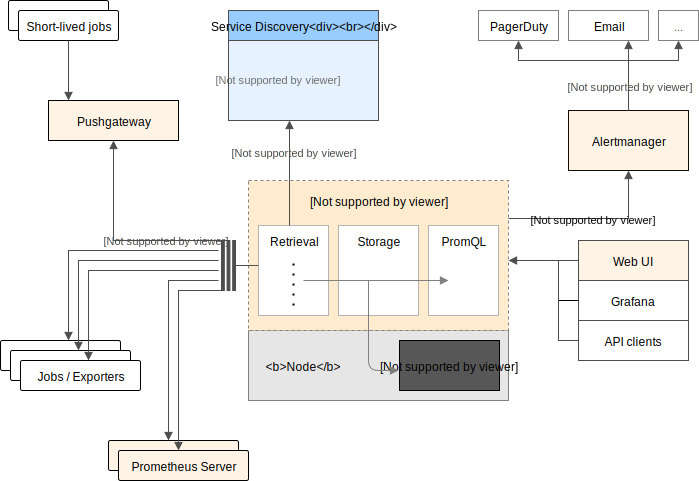
\includegraphics[width=0.55\linewidth]{architecture}
			\caption{Architectura prometheusa}
			\label{fig:architecture}
		\end{figure}
\end{frame}
\begin{frame}[fragile]{Konfiguracja serwera - joby}
	\begin{verbatim}
scrape_configs:		
  - job_name: 'prometheus'
    static_configs:
    - targets: ['localhost:9090']		
  - job_name: 'jumping-turtle'
    metrics_path: /actuator/prometheus
    static_configs:
      - targets: ['coreos05.wyborcza.pl:8081', 'localhost:8080']
	  - labels:
        service: jumping-turtle
	\end{verbatim}
\end{frame}
\begin{frame}[fragile]{Alerty}
	\begin{verbatim}
		rule_files:
		  - "alerts.rules.yml"		  
	\end{verbatim}
	Alerty:
	\begin{verbatim}
	alerting:
	  alertmanagers:
	    - static_configs:
	      - targets: ['localhost:9093']
	\end{verbatim}
\end{frame}
\section{Rodzaje metryk}
\begin{frame}{Rodzaje metryk}
	\begin{itemize}
		\item Licznik - funkcja niemalejąca
		\item Gaugage - konkrentne wartości
		\item histogram - pakiety po x próbek
		\item Summary - okno czasowe
	\end{itemize}
\end{frame}
\section{Agregacja, Alerty i jak używać metryk}
\begin{frame}[fragile]{POM}
	\begin{lstlisting}[language=XML]
<dependency>
  <groupId>io.micrometer</groupId>
  <artifactId>micrometer-registry-prometheus</artifactId>
  <version>${micrometer.version}</version>
</dependency>
	\end{lstlisting}
\end{frame}
\begin{frame}[fragile]{Obsługa annotacji @Timed}
		\begin{lstlisting}
@Bean
public TimedAspect timedAspect(MeterRegistry registry) {
	return new TimedAspect(registry);
}
		\end{lstlisting}
\end{frame}
\end{document}